\documentclass[16pt]{beamer}
% \geometry{papersize={5in,4.5in}}

\ifdefined\chinchin
\usepackage[CJKspace]{xeCJK}
%\setCJKmainfont[BoldFont=SimHei,ItalicFont=AR PL KaitiM GB]{Alibaba PuHuiTi}
\setCJKmainfont{Alibaba PuHuiTi}
\newcommand{\cc}[2]{#1}
\else
\newcommand{\cc}[2]{#2}
% \renewcommand{\baselinestretch}{0.8}
\fi

%\usepackage{newtxtext,newtxmath}	% use Times Roman font
%\usepackage{newtxtext}
%\renewcommand{\familydefault}{\sfdefault}
\usefonttheme{serif}
\usefonttheme{professionalfonts}
%\setbeamertemplate{theorems}[numbered]
\setbeamertemplate{caption}{\insertcaption} 	% no `Figure' prefix before caption

\mode<presentation> {

%\usetheme{default}
%\usetheme{AnnArbor}
%\usetheme{Antibes}
%\usetheme{Bergen}
%\usetheme{Berkeley}
%\usetheme{Berlin}
%\usetheme{Boadilla}
%\usetheme{CambridgeUS}
%\usetheme{Copenhagen}
%\usetheme{Darmstadt}
%\usetheme{Dresden}
%\usetheme{Frankfurt}
%\usetheme{Goettingen}
%\usetheme{Hannover}
%\usetheme{Ilmenau}
%\usetheme{JuanLesPins}
%\usetheme{Luebeck}
\usetheme{Madrid}
%\usetheme{Malmoe}
%\usetheme{Marburg}
%\usetheme{Montpellier}
%\usetheme{PaloAlto}
%\usetheme{Pittsburgh}
%\usetheme{Rochester}
%\usetheme{Singapore}
%\usetheme{Szeged}
%\usetheme{Warsaw}

%\usecolortheme{albatross}
%\usecolortheme{beaver}
%\usecolortheme{beetle}
%\usecolortheme{crane}
%\usecolortheme{dolphin}
%\usecolortheme{dove}
%\usecolortheme{fly}
%\usecolortheme{lily}
\usecolortheme{orchid}
%\usecolortheme{rose}
%\usecolortheme{seagull}
%\usecolortheme{seahorse}
%\usecolortheme{whale}
%\usecolortheme{wolverine}		% Hofstra

%\setbeamertemplate{footline} % To remove the footer line in all slides uncomment this line
\setbeamertemplate{footline}[page number] % To replace the footer line in all slides with a simple slide count uncomment this line
\setbeamertemplate{navigation symbols}{} % To remove the navigation symbols from the bottom of all slides uncomment this line
}

\setbeamertemplate{headline}{}
% \setbeamersize{text margin left=1mm,text margin right=1mm}
% \settowidth{\leftmargini}{\usebeamertemplate{itemize item}}
% \addtolength{\leftmargini}{\labelsep}
% \setbeamertemplate{enumerate subitem}{(\roman{enumii})}
% \setbeamertemplate{itemize items}[default]
\setbeamertemplate{items}[square]
\setbeamertemplate{enumerate items}[default]

\usepackage[backend=biber,style=numeric]{biblatex}
\bibliography{../AGI-book}
% \renewcommand*{\bibfont}{\footnotesize}
\setbeamertemplate{bibliography item}[text]

\usepackage{graphicx} % Allows including images
\usepackage{tikz-cd}
\usetikzlibrary{decorations.pathmorphing}
% \usepackage{tikz}
\usepackage[export]{adjustbox}% http://ctan.org/pkg/adjustbox
\usepackage{verbatim} % comments
\usepackage[skins,theorems]{tcolorbox}

\usepackage{ulem}
\makeatletter
\newcommand{\cthickuline}[3][0.5pt]{%
	\UL@protected\def\temp@uline{\bgroup\markoverwith
		{\textcolor{#2}{\rule[-0.5ex]{2pt}{#1}}}\ULon}%
	\temp@uline{#3}%
}
\makeatother

% \usepackage{tikz-cd}  % commutative diagrams
% \newcommand{\tikzmark}[1]{\tikz[overlay,remember picture] \node (#1) {};}
% \usepackage{booktabs} % Allows the use of \toprule, \midrule and \bottomrule in tables
% \usepackage{amssymb}  % \leftrightharpoons
% \usepackage{wasysym} % frownie face
% \usepackage{newtxtext,newtxmath}	% Times New Roman font
% \usepackage{sansmath}

\let\oldtextbf\textbf
\renewcommand{\textbf}[1]{\textcolor{blue}{\oldtextbf{#1}}}
\newcommand{\emp}[1]{\textbf{\color{violet}#1}}

\newcommand{\vect}[1]{\boldsymbol{#1}}
\newcommand{\tab}{\hspace*{1cm}}
\newcommand*\confoundFace{$\vcenter{\hbox{\includegraphics[scale=0.2]{../confounded-face.jpg}}}$}
\newcommand{\smiley}{$\vcenter{\hbox{\includegraphics[scale=0.05]{../smiling-face.png}}}$}
\newcommand{\cubic}{\vcenter{\hbox{\includegraphics[scale=1]{../cubic-symbol.png}}}}

\makeatletter
\renewcommand{\boxed}[1]{\fbox{\m@th$\displaystyle\scalebox{0.9}{#1}$} \,}
\makeatother

%----------------------------------------------------------------------------------------
%	TITLE PAGE
%----------------------------------------------------------------------------------------

\title[AGI-aaS]{Strong AI as a Service}
\author{YKY}
\date{\today} % Date, can be changed to a custom date

\begin{document}

\addtocounter{page}{-1}
\begin{frame}[plain,noframenumbering]
\titlepage
\end{frame}

\addtocounter{page}{-1}
\begin{frame}[noframenumbering]
\frametitle{Contents}
\fontsize{10pt}{8}\selectfont
% blah table of contents...

\begin{enumerate}[I]
	\item Technical Details
		\begin{enumerate}[1]
			\item How is AGI different from LLMs?
			\item Logic Transformers
		\end{enumerate}
	\item Political-Economic Analysis
		\begin{enumerate}[1]
			\item "Convergence"
			\item American Hegemony
		\end{enumerate}
\end{enumerate}
\end{frame}

%----------------------------------------------------------------------------------------
%	PRESENTATION SLIDES
%----------------------------------------------------------------------------------------

\part{Technical Details}
\frame{\partpage}

\begin{frame}
\frametitle{How is AGI different from LLMs?}
	\begin{itemize}
		\item Reinforcement learning is like a loop.  Its ``knowledge'' changes slowly over many cycles.  Think of it like a washing-machine rinsing out dirt in the clothes.
		\begin{center}
			
\includegraphics[scale=0.1]{washing-machine.png}
		\end{center}
		\item Over many cycles, the knowledge in the machine gets more and more correct, removing internal contradictions.
		\item This is how to solve the problem of \textbf{hallucinations}.
		\item LLM: more bulky \qquad AGI: more compact
	\end{itemize}
\end{frame}

\begin{frame}
	\frametitle{Logic Transformers}
	\begin{itemize}
		\item Differentiable.
		\item Cylindrification factor.
		\item I was in quite a celebratory mood, as you can see.
		\item The source code is open under Creative Common license, so you can ask Copilot whether our project has genuine original value
	\end{itemize}
\end{frame}

\begin{frame}
	\begin{center}
		
\includegraphics[scale=0.45]{logic-Transformer-string-diagram.png}
	\end{center}
\end{frame}

\part{Political-Economic Analysis}
\frame{\partpage}

% 找出更好地說故事的方式。

\begin{frame}
	\frametitle{The AGI ethics problem is even harder than AGI}
	\begin{itemize}
		\item American hegemony 令 冇啖好食 $\rightarrow$ 務必消除種族歧視，乃大勢之所趨
		\item Curse of backwardness: 中國無法改革之迷思 $\rightarrow$ 落後的解決方案
		\item Metamorphosis: AGI 勢將導致人類物種之蛻變，所以不可懼怕鉅變
		\item 除了趨向絕對真理，別無其他的 anchor
		\item 嘗試以香港爲基地 建立 中立 AGI server
	\end{itemize}
\end{frame}

\begin{frame}
	\frametitle{Our Core values}
	\begin{center}
		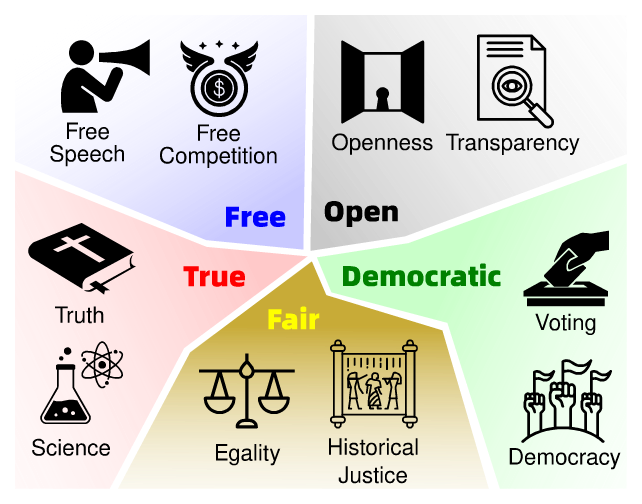
\includegraphics[scale=1]{DAO-principles.png}
	\end{center}
\end{frame}

\begin{frame}
\frametitle{References}
\cc{多谢收看}{Thanks for watching} \smiley \vspace{1cm}
\printbibliography
\end{frame}

\end{document}